\section{2. Time-Independent Schr\"{o}dinger Equation} \hrule height 0.3pt \thinspace

\subsection{\underline{2.1 Stationary States}}
Suppose PE is independent of time, $V(\vec{r}, t) = V(\vec{r})$. \\
Separation of variables: $\Psi(\vec{r}, t) = \psi(\vec{r}) \varphi(t)$ \\

Eq of motion for $\varphi(t)$: $\varphi(t) = e^{-iEt/\hbar}$ \\

Eq of motion for $\psi(\vec{r})$ is the time-independent Schr\"{o}dinger equation:
$$-\frac{\hbar^2 }{2m} \dv[2]{\psi(\vec{r})}{x} + V(\vec{r}) \psi(\vec{r}) = E \psi(\vec{r}) $$ \\

TD of the wavefunction that corresponds to the constant $E$ is easily written once we solve the TISE: $\Psi_{E}(\vec{r}, t) = \psi_{E}(\vec{r}) e^{-iEt / \hbar}$ \\

\medskip

Properties of solutions for TI potentials: \\

\begin{itemize}[noitemsep,wide=0pt, leftmargin=\dimexpr\labelwidth + 2\labelsep\relax]
    \item \textbf{The constant $E$ must be real.}
    
    \item \textbf{Stationary wavefunction.} \\
        $\mathcal{P}(\vec{r}, t) = |\psi_E(\vec{r}, t)|^2 = |\psi_E(\vec{r})|^2$ (TD cancels out).

    \item \textbf{Stationary wavefunction is a state of definite energy.} \\
        The total energy (kinetic plus potential) is the Hamiltonian: $H(x, p) = \frac{p^2}{2m} + V(x)$. \\

        Hamiltonian operator: $\widehat{H} = -\frac{\hbar^2}{2m} \pdv[2]{}{x} + V(x)$ \\
        Thus the TISE can be written as $\widehat{H} \psi = E \psi$ \\

        $\langle \widehat{H} \rangle = E$, $\langle \widehat{H} ^2 \rangle = E^2$, $\Delta E = \sqrt{\langle \widehat{H}^2 \rangle - \langle \widehat{H} \rangle ^2} = 0$

    \item Spatial part of stationary wavefunction can be chosen to be real. \\
        $\psi^*(\vec{r})$ is a soln w/ same $E$ \\
        Solns can be chosen to be real: $\psi(\vec{r}) + \psi^*(\vec{r})$ and $\frac{\psi(\vec{r}) - \psi^*(\vec{r})}{i}$.

    \item \textbf{Parity symmetry: even and odd wavefunctions.}
        Suppose $V(-\vec{r}) = V(\vec{r})$. Then, $\psi_E(-\vec{r})$ is a soln w the same energy. \\
        $\psi_E(\vec{r}) + \psi_E(-\vec{r})$ is even under reflection, $\psi_E(\vec{r}) - \psi_E(-\vec{r})$ is odd. \\
        When the potential is symmetric under reflection, we can choose the stationary states to be either even or odd under reflection.

    \item \textbf{Orthogonality/orthonormality.} \\
        $\int \psi_m (\vec{r})^* \psi_n (\vec{r}) d^3 \vec{r} = \delta_{mn}$ where $\delta_{mn}$ is 0 if $m \neq n$ and 1 if $m = n$.

    \item \textbf{Linearity.} \\
        The SE is linear. Given stationary states, a linear combo of these
            $$\psi(\vec{r}, t) = \sum_{n} c_n \psi_n(\vec{r}, t) = \sum_n c_n \psi_n(\vec{r}) e^{-\frac{i}{\hbar} E_n t}$$
        where $c_n$ are complex constants, is a solution to the TDSE 
        $$i \hbar \pdv{\psi(\vec{r}, t)}{t} = \widehat{H} \psi(\vec{r}, t)$$

    \item \textbf{Time evolution.}
        Given $$\psi(\vec{r}, 0) = \sum_n c_n \psi_n(\vec{r}, 0) = \sum_n c_n \psi_n (\vec{r})$$
        at time $t$, the time evolution is 
        $$\psi(\vec{r}, t) = \sum_n c_n \psi_n(\vec{r}, t) = \sum_n c_n \psi_n(\vec{r}) e^{-\frac{i}{\hbar} E_n t}$$

        Once we've expanded a given initial wavefunction in terms of a linear combo of the stationary wavefunctions $\psi_n(\vec{r})$, the time evolution follows simply by putting a factor of $e^{-i/\hbar E_n t}$ to each term containing $\psi_n(\vec{r})$.

    \item \textbf{Normalization.} \\
        The constant coefficients are constrained by $\sum_n |c_n|^2 = 1$

    \item \textbf{Completeness.} \\
        The stationary states form a complete set if
            $$\sum_n \psi_n (\vec{r'}, t)^* \psi_{n} (\vec{r}, t) = \delta^3 (\vec{r'} - \vec{r})$$

        where $\delta^3(\vec{r'} - \vec{r})$ is the Dirac-delta function in 3D defined by $$\int d^3 \vec{r'} \psi(\vec{r'}, t) \delta^3(\vec{r'} - \vec{r}) = \psi(\vec{r}, t)$$
\end{itemize}

\textbf{Euler's formula}: $e^{i \theta} = \cos \theta + i \sin \theta$ \\
\textbf{sin and cos}: $\cos(\theta) = \frac{1}{2}(e^{i \theta} + e^{-i \theta})$, $\sin(\theta) = \frac{1}{2}(e^{i \theta} - e^{-i \theta})$ \\

\textbf{Delta function}: Given $f(x)$, $\delta(x - x')$ is defined as $f(x') = \int f(x) \delta(x - x') dx$ \\
$\int \delta(x - x') dx = 1$, note this is not the area \\

    $\delta_{\alpha}(x) = \frac{1}{\alpha \sqrt{\pi}} e^{-\frac{x^2}{\alpha^2}}$,
    $\delta_{\alpha}(x) = \frac{1}{\pi x} \sin(\frac{x}{a})$, 
    $\delta_{\alpha}(x) = \frac{\alpha}{\pi x^2} \sin^2 (\frac{x}{\alpha})$ \\

\subsection{\underline{One-dimensional systems}}
Wavefunction for a system containing a single particle of mass $m$ in 1D with TI potentials.
    $$- \frac{\hbar^2}{2m} \dv[2]{\psi(x)}{x} + V(x) \psi(x) = E \psi(x)$$

Once we find the wavefunction $\psi_E(x)$ of energy $E$, its time dependence follows easily:
    $$\psi_E(x, t) = \psi_E(x) e^{-\frac{i}{\hbar} E t}$$

\textbf{Boundary conditions} \\
1. When the potential $V(x)$ has a finite jump at $x = a$, both $\psi(x)$ and $\psi'(x)$ are continuous across $x = a$. \\
2. When the potential $V(x)$ has an infinite jump at $x = a$, $\psi(x)$ is continuous but $\psi'(x)$ is discontinuous across $x = a$.

Futhermore, the wavefunction must vanish at $x = \pm \infty$ for a normalizable wavefunction.

\subsection{\underline{2.2 The Infinite Square Well}}
    $$V(x) = \begin{cases} 0, \textrm{if } 0 \leq x \leq a \\ \infty, \textrm{otherwise} \end{cases}$$

    $$\psi(x) = 0 \textrm{ for } x < 0 \textrm{ and } x > a$$
For $0 \leq x \leq a$, $V(x) = 0$ and the Schr\"odinger equation reduces to 
    $$\psi''(x) + k^2 \psi(x) = 0 \textrm{, where } k = \sqrt{\frac{2mE}{\hbar^2}} \textrm{ and } E > 0$$

Classic \textbf{simple harmonic oscillator}: $\psi(x) = A \sin(kx) + B \cos(kx)$ \\

\textbf{Boundary conditions}: \\
Continuity of $\psi(x)$ at $x = 0$ sets $\psi(0) = B = 0 \rightarrow \psi(x) = A \sin(kx)$ \\
at $x = a$ sets $\psi(a) = A \sin(ka) = 0$

$$k_n = \frac{n \pi}{a}, n = 1, 2, ...$$

$$\psi_n(x) = \sqrt{\frac{2}{a}} \sin(\frac{n \pi}{a} x) \qquad E_n = \frac{\hbar^2 k_n^2}{2m} = \frac{n^2 \pi^2 \hbar^2}{2ma^2}$$

$\psi_1$ is the ground state, others are excited states. \\

Properties of $\psi_n(x)$: \\
1. Alternatively even and odd. \\
2. As you go up in energy, each successive state has one more node. \\
3. They are mutually orthogonal, in the sense that $\int \psi_m(x)* \psi_n(x) dx = 0$ whenever $m \neq n$. \\

$\int \psi_m (x)* \psi_n(x) dx = \delta_{mn}$
where $\delta_{mn}$ (Kronecker delta) is 0 if $m \neq n$ and 1 if $m=n$. We say that the $\phi$'s are orthonormal.

4. They are complete, in the sense that any other function, $f(x)$, can be expressed as a linear combination of them (Fourier series), Dirichlet's theorem:
    $$f(x) = \sum_{n=1}^{\infty} c_n \psi_n(x) = \sqrt{\frac{2}{a}} \sum_{n=1}^{\infty} c_n \sin(\frac{n \pi}{a} x)$$

Fourier's trick: $c_n = \int \psi_n(x)^* f(x) dx$ \\
$$c_m = \frac{2}{a} \int_0^a f(x) \sin(\frac{m \pi x}{a}) dx$$

$|c_n|^2$ tells you the probability that a measurement of the energy would yield the value $E_n$. \\

Sum of these probabilities should be 1: 
    $$\sum_{n=1}^{\infty} |c_n|^2 = 1$$

The expectation value of the energy is
    $$\langle H \rangle = \sum_{n=1}^{\infty} |c_n|^2 E_n$$

Conservation of energy in QM

\subsection{\underline{2.3 The Harmonic Oscillator}}
Hooke's law (mass $m$ w/ spring constant $k$): $F = -kx = m \frac{d^2 x}{d t^2}$ \\
Solution is $x(t) = A \sin(\omega t) + B \cos(\omega t)$, where $\omega = \sqrt{\frac{k}{m}}$ \\
Potential energy: $V(x) = \frac{1}{2} k x^2 = \frac{1}{2} m \omega^2 x^2$ \\

Expanding $V(x)$ in a \textbf{Taylor series} about the min: $V(x) = V(x_0) + V'(x_0) (x - x_0) + \frac{1}{2} V''(x_0)(x- x_0)^2 + \cdots$ \\
Simple harmonic oscillaton, $V(x) \cong \frac{1}{2} V''(x_0) (x - x_0)^2, k = V''(x_0)$

The Schr\"{o}diner Equation for the harmonic oscillator: $$-\frac{\hbar^2}{2m} \dv[2]{\psi}{x} + \frac{1}{2} m \omega^2 x^2 \psi = E \psi$$ \\

Boundary conditions: $\psi(-\infty) = 0, \qquad \psi(+\infty) = 0$

\medskip

\textit{\underline{1. Simplify notation with change of variables}} \\
Introduce $\xi \equiv \sqrt{\frac{m \omega}{\hbar}} x$. \\
SE becomes $\dv[2]{\psi}{\xi} = (\xi^2 - K) \psi$, where $K \equiv \frac{2E}{\hbar \omega}$. \\

\textit{\underline{2. Asymptotic behavior}} \\

Working in the large $\xi^2 >> K$ region, \\
\textbf{Hermite eqn}: $H''(\xi) - 2 \xi H'(\xi) + (K - 1) H(\xi) = 0$ \\

\textbf{Hermite polynomials}: $H_0 = 1$, $H_1 = 2 \xi$, $H_2 = 4 \xi^2 - 2$, $H_3 = 8 \xi^3 - 12 \xi$, $H_4 = 16 \xi^4 - 48 \xi^2 + 12$, $H_5 = 32 \xi^5 - 160 \xi^3 + 120 \xi$ \\

\textit{\underline{3. Method of power series}}

\begin{vwcol}[widths={0.7,0.3},sep=.1cm,rule=0pt,indent=0em]

The recursion formula: $a_{j+2} = \frac{(2j + 1 - K)}{(j + 1)(j + 2)} a_j$ \\
Recursion formula for allowed $K$: \\ $a_{j+2} = \frac{-2(n - j)}{(j+1)(j+2)} a_j$ \\

$h(\xi) = a_0 + a_1 \xi + a_2 \xi^2 + \cdots = \sum_{j=0}^{\infty} a_j \xi^j$ \\
$h(\xi) = h_{\text{even}}(\xi) + h_{\text{odd}}(\xi)$ \\

\columnbreak

\vspace{-1em}
\begin{Figure}
    \raggedright
    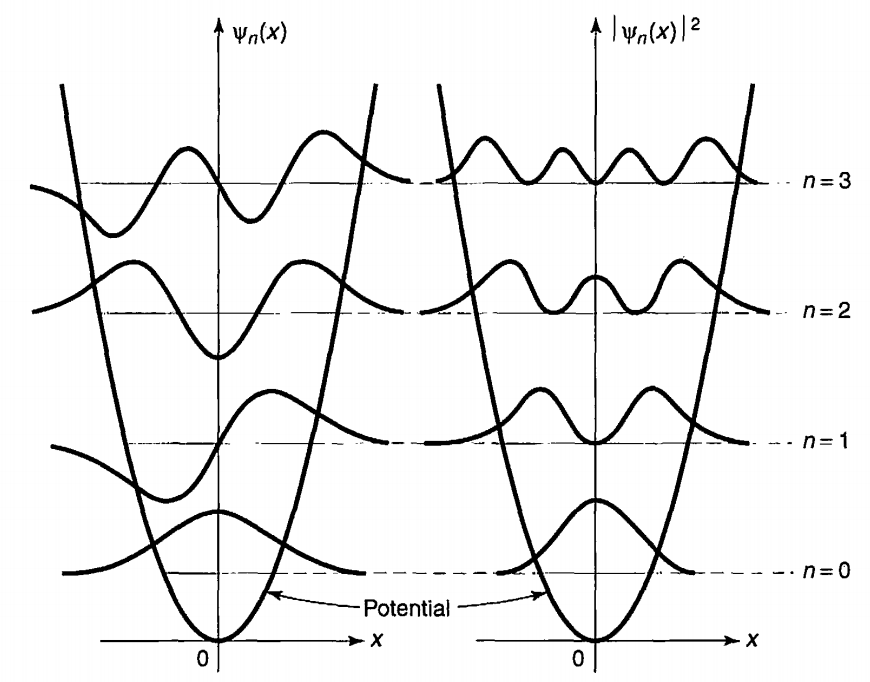
\includegraphics[width=0.3\columnwidth]{figures/harmonic_oscillator1.png}
\end{Figure}
\vspace{-1em}

\end{vwcol}

\textit{\underline{4. Infinite series produces a diverging function}} \\

For large $n$, we have $a_{n+2} \approx \frac{2}{n} a_n$ 

\textit{\underline{5. Truncate series}}

\begin{vwcol}[widths={0.8,0.2},sep=0cm,rule=0pt,indent=0em]

$K = 2n + 1$, so $E_n = (n + \frac{1}{2}) \hbar \omega$ \\
The normalized stationary states: \\
$\psi_n(x) = (\frac{m \omega}{\pi \hbar})^{1/4} \frac{1}{\sqrt{2^n n!}} H_n(\xi) e^{-\xi^2 / 2}$ \\

Rodrigues formula: $H_n(\xi) = (-1)^n e^{\xi^2} (\dv{}{\xi})^n e^{-\xi^2}$

\columnbreak

\vspace{-1em}
\begin{Figure}
    \raggedright
    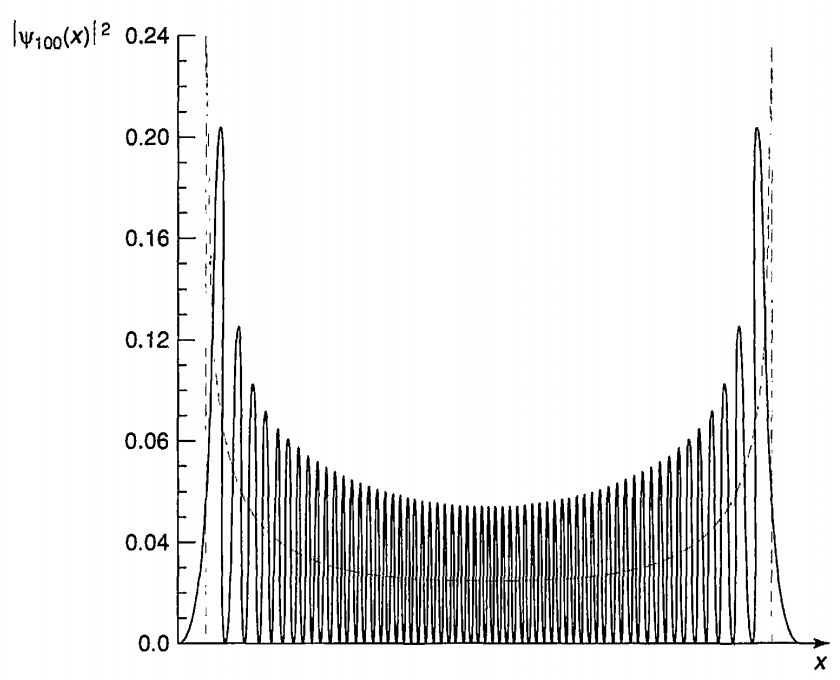
\includegraphics[width=0.2\columnwidth]{figures/harmonic_oscillator2.png}
\end{Figure}
\vspace{0em}

\end{vwcol}

\subsection{\underline{2.4 The Free Particle}}
$$\pdv[2]{\xi}{x} = -k^2 \xi, k = \frac{\sqrt{2mE}}{\hbar}$$

General solution to the TISE: wave packet, $\Psi(x, t) = \frac{1}{\sqrt{2\pi}} \int_{-\infty}{\infty} \psi(k) e^{i (kx - \frac{\hbar k^2}{2m} t)} dk$ \\
$$\phi(x) = \frac{1}{\sqrt{2 \pi}} \int_{-\infty}^{+\infty} \Psi(x, 0) e^{-ikx} dx$$

Plancherel's theorem: $$f(x) = \frac{1}{\sqrt{2 \pi}} \int_{-\infty}^{\infty} F(k) e^{ikx} dk \leftrightarrow F(k) = \frac{1}{\sqrt{2\pi}} \int_{-\infty}^{\infty} f(x) e^{-kx} dx$$

$F(k)$ is the Fourier transform of $f(x)$; $f(x)$ is the inverse Fourier transform of $F(k)$ \\

Phase velocity: speed of individual ripples; group velocity: speed of the envelope \\

Dispersion relation: the formula for $\omega$ as a function of $k$

\subsection{\underline{2.5 The Delta-Function Potential}}

\textbf{Dirac delta function} is an infinitely high, infinitesimally narrow spike at the origin, whose area is 1:

    $$\delta(x) = \begin{cases} 0, \textrm{if } x \neq 0 \\ \infty, \textrm{if } x = 0 \end{cases}$$

$f(x) \delta(x - a) = f(a) \delta(x - a)$ bc the product is 0 anyway except at $a$. \\

In particular, $\int_{-\infty}^{\infty} f(x) \delta(x-a) dx = f(a)$. $a - \epsilon$ to $a + \epsilon$ would do, for any $\epsilon > 0$.

Consider $V(x) = -\alpha \delta(x)$, where $\alpha$ is some positive constant. \\

$$-\frac{\hbar^2}{2m} \dv[2]{\psi}{x} - \alpha \delta(x) \psi = E \psi$$

\textit{Bound states (E < 0)}: \\

\textit{Scattering states (E > 0)}: \\

%For $x < 0$ the SE reads $$\dv[2]{\psi}{x} = -\frac{2mE}{\hbar^2} \psi = -k^2 \psi$$


\subsection{\underline{2.6 The Finite Square Well}}
$V(x) = \begin{cases} -V_{0}, \textrm{for } -a < x < a \\ 0, \textrm{for } |x| > a \end{cases},$ 

\vspace{-5em}
\begin{Figure}
    \raggedleft
    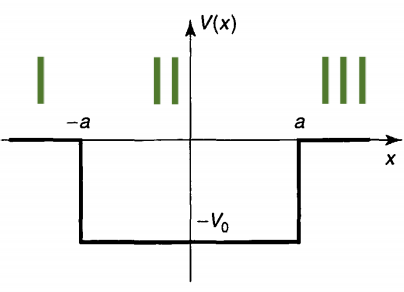
\includegraphics[width=0.3\columnwidth]{figures/finite_square_well.png}
\end{Figure}
\vspace{-2em}

where $V_0$ is a positive constant.

Both bound states ($E < 0$) and scattering states ($E > 0$). \\

\textit{\underline{Bound states}}: \\
Potential is piecewise and discontinuous, can split into regions. \\

\textbf{\textit{REGION I}}
$$-\frac{\hbar}{2m} \dv[2]{\psi}{x} = E \psi, \textrm{ or } \psi''_{I}(x) - \kappa^2 \psi_{I}(x) = 0, \qquad \kappa \equiv \sqrt{-\frac{2mE}{\hbar}}$$
where $E < 0$ for a bound state. \\
General sol: $\psi_{I}(x) = Ae^{-\kappa x} + B e^{\kappa x}$. \\
$x = -\infty \rightarrow \psi(x) = 0$, so $A = 0$, and we have $\psi_{I}(x) = Be^{\kappa x}$

\smallskip

\textbf{\textit{REGION II}} \\
$$-\frac{\hbar^2}{2m} \dv[2]{\psi}{x} - V_0 \psi = E \psi, \textrm{ or } \psi'' = -l^2 \psi, \qquad l \equiv \sqrt{\frac{2m (E + V_0)}{\hbar}}$$

General sol: $\psi(x) = C \sin(lx) + D \cos(lx)$, for $-a < x < a$

\smallskip

\textbf{\textit{REGION III}} \\
SE and general sol same as region I, but $x = \infty \rightarrow \psi(x) = 0$, so $G=0$ and $\psi_{III}(x) = Fe^{-\kappa x}$

\medskip
\hrule height 0.3pt \thinspace

\textbf{Even bound states} \\
$\psi(-x) = \psi(x)$, $\psi_{II}(x) = D \cos(lx)$ \\
Bc the potential has only a finite discontinuity at $x = \pm a$, both $\psi$ and $\psi'$ must be continuous at $x = \pm a$.

$x = a$, $\psi_{II}(a) = \psi_{III}(a)$ imposes $D \cos(la) = F e^{-\kappa a}$ \\

$x = a$, $\psi'_{II}(a) = \psi'_{III}(a)'$ imposes $-lD \sin(la) = -\kappa F e^{-\kappa a}$ \\

Continuity of $\psi(x)$ and $\psi'(x)$ at $x = -a$ does not add anything new. \\

Dividing the above two, we get $\kappa = l \tan(la)$ \\
This is a formula for the allowed energies, since $\kappa$ and $l$ are both functions of $E$. Let $z \equiv la$, and $z_0 \equiv \frac{a}{\hbar} \sqrt{2m V_0}$. $\kappa^2 + l^2 = 2m V_0 / \hbar^2$, so $\kappa a = \sqrt{{z_0}^2 - z^2}$. \\

Transcendental eq for $z$ (and hence $E$) as a function of $z_0$ (which is a measure of size of well): $\tan z = \sqrt{(\frac{z_0}{z})^2 - 1}$

\textbf{Odd bound states} \\
$\psi_{II}(x) = C \sin(lx)$ \\

$x = -a, \psi_{II}(-a) = \psi_{I}(-a)$ imposes $C \sin(la) = B e^{-\kappa a}$ \\
$x = -a, \psi'_{II}(-a) = \psi'_{I}(-a)$ imposes $l C \cos(la) = -\kappa B e^{-\kappa a}$ \\

Dividing the above two, $l \cot(la) = -\kappa$. \\
Rewriting this in terms of $z$ and $z_0$, $$\cot(z) = - \sqrt{(\frac{z_0}{z})^2 - 1}$$

$V_{1}$ does not support an odd bound state, since there is no intersection pt, $V_{2}$ produces only one bound state, and $V_{3}$ produces two bound states. Finite well potential supports at least one even state, the ground state, and it may not support any of the excited states.

\vspace{0em}
\begin{Figure}
    \raggedright
    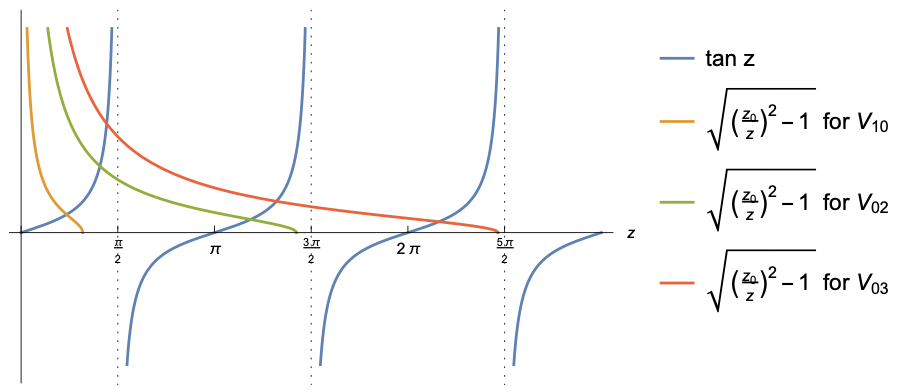
\includegraphics[width=0.5\columnwidth]{figures/even_finite_square_well.png}
\end{Figure}
\vspace{-1em}

\vspace{-9em}
\begin{Figure}
    \raggedleft
    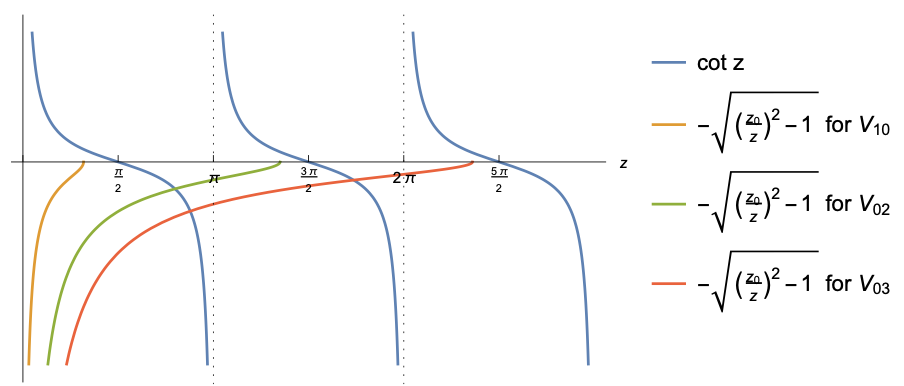
\includegraphics[width=0.5\columnwidth]{figures/odd_finite_square_well.png}
\end{Figure}
\vspace{-1em}

\medskip
\hrule height 0.3pt \thinspace

\textbf{Wide and deep well} \\

\begin{vwcol}[widths={0.6,0.4},sep=.1cm,rule=0pt,indent=0em] 
$z_n \approx \frac{n \pi}{2}, n = 1, 2, 3, ...$. \\

Using the def of $z$ and solving for $E$, 
$E_n = -V_0 + \frac{\hbar^2 \pi^2 n^2}{2m(2a)^2}, n = 1, 2, ...$

Thus, the energy levels of the infinite square well of width $2a$ are reproduced for $E_n - (-V_0) = E_n + V_0$, which is the energy above the bottom of the well. As $V_0 \rightarrow \infty$, finite sq well goes to infinite sq well.

\columnbreak

\vspace{-1em}
\begin{Figure}
 \raggedright
 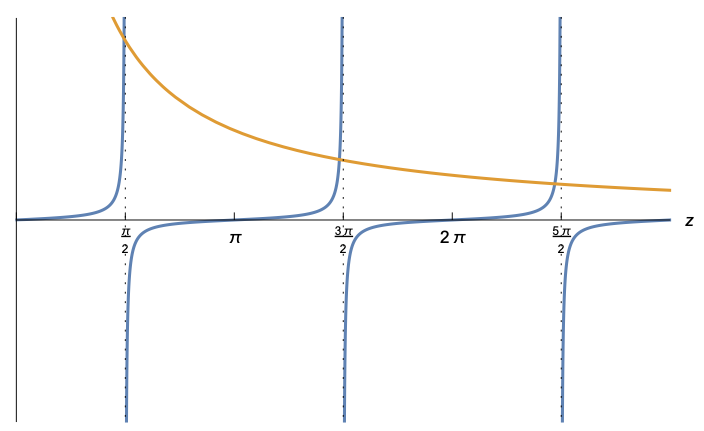
\includegraphics[width=0.4\columnwidth]{figures/wide_deep_finite_square_well.png}
\end{Figure}
\vspace{-1em}

\end{vwcol}

\textbf{Shallow and narrow well} \\
Any shallow or narrow well supports at least one bound state. But we need at least $z_0 = \sqrt{\frac{2mV_0 a^2}{\hbar^2}} \geq \frac{\pi}{2}$ to support any odd state.

\subsection{\underline{Gaussian integrals}}
$$\int_{-\infty}^{\infty} e^{-ax^2} dx = \sqrt{\frac{\pi}{a}} \textrm{ and } \int_{0}^{\infty} e^{-ax^2} dx = \frac{1}{2} \sqrt{\frac{\pi}{a}}$$
$$\int_{-\infty}^{\infty} x^{2n+1} e^{-ax^2} dx = 0 \textrm { for } n = 0, 1, 2, ...$$
$$\int_{-\infty}^{\infty} x^{2n} e^{-ax^2} dx = (-1)^n \dv[n]{}{a} \sqrt{\frac{\pi}{a}} \textrm{ for } n = 0, 1, 2, ...$$
$$\int_{-\infty}^{\infty} e^{-ax^2 + bx} dx = \sqrt{\frac{\pi}{a}} e^{\frac{b^2}{4a}}  \qquad  \int_{-\infty}^{\infty} x^n e^{-ax^2 + bx} dx = \dv[n]{}{b} \sqrt{\frac{\pi}{a}} e^{\frac{b^2}{4a}}$$

